%! TEX root = ../main.tex
\documentclass[main]{subfiles}

\begin{document}
\chapter{実験4:代理モデル導入時の最適化}
    \section{目的}
    これまでの章で,長野市バス運行スケジュール最適化問題の高速化のために,
    Walsh関数による代理モデルを使用するために必要な要素を決定した.
    本章では,これらの情報を用いて,実際に最適化問題に代理モデルを導入し,高速化が達成できているか検証する.
    ここで,代理モデルを導入した最適化を行った時,どのような結果を得ることが出来れば,高速化が達成できたと言えるのかを確認する.
    図\ref{hv_plot_}は,先行研究でのバス利用率4.5\%の時の世代数ごとのHVを表す.これは図\ref{hv_plot}と同一である.
    
    \begin{figure}
        \centering
        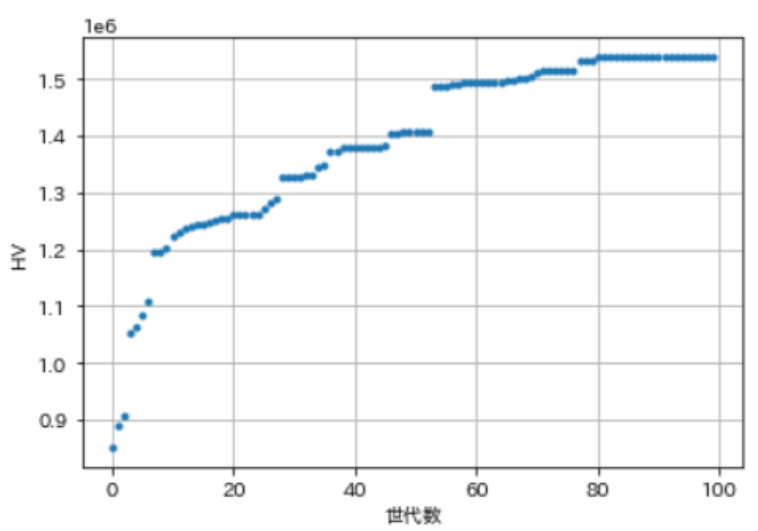
\includegraphics[width=\linewidth]{figures/hv_plot.png}
        \caption{バス利用率4.5\%の場合のHV推移}
        \label{hv_plot_}
    \end{figure}
    先行研究では100世代まで最適化を行い,そのHVが$1.538\times 10^6$であった.
    つまり,代理モデルを導入して最適化を行った結果,
    \begin{itemize}
        \item 100世代目のHVが$1.538\times 10^6$を超える
        \item 100世代目までにHVが$1.538\times 10^6$を超える
    \end{itemize}
    この2つのどちらかを満たしたとき,代理モデルによって最適化を高速化することが出来たと言える.
    
    また,先行研究で使用したアルゴリズムのフローチャートを図\ref{old_algo}に示す.
    \begin{figure}
        \centering
        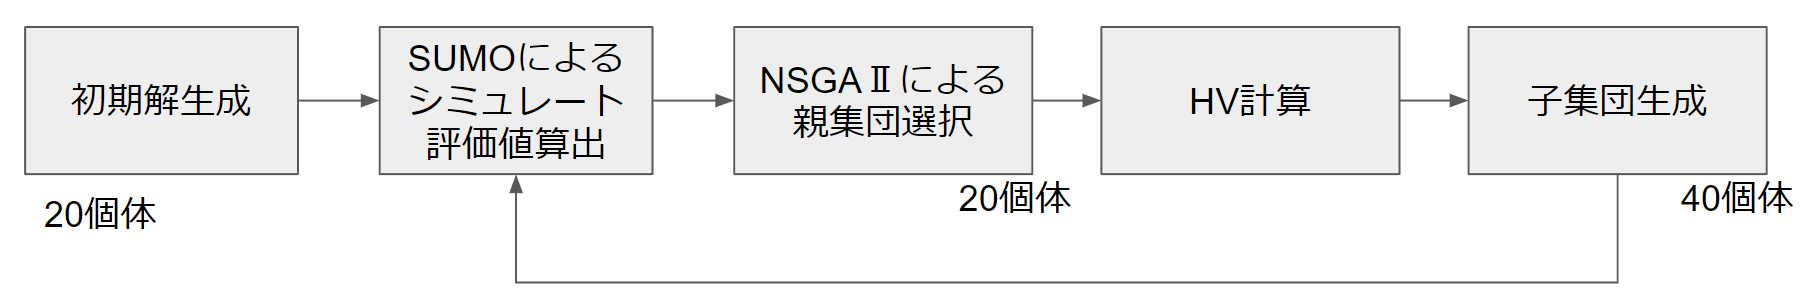
\includegraphics[width=\linewidth]{figures/old_algo.png}
        \caption{先行研究でのアルゴリズムのフローチャート}
        \label{old_algo}
    \end{figure}
    初期解を20個体生成させる.次に,HVを計算し,子集団を20個体生成する.
    新しい解である子集団20個体に対してSUMOによるシミュレートを行い評価値を算出する.
    親集団と子集団合わせた40個体に対し,NSGAⅡにより優れた解20個体を選択する.選ばれた20個体を親集団とする.
    このループを1世代として,ループを100回行うのが先行研究のアルゴリズムである.

    \section{実験方法}
    代理モデルの導入方法について2つの手法を提案する.
    以下でその2つについて,提案手法のフローチャートと特徴について述べる.
        \subsection{提案手法1}
        図\ref{d}にフローチャートを示す.
        \begin{figure}
            \centering
            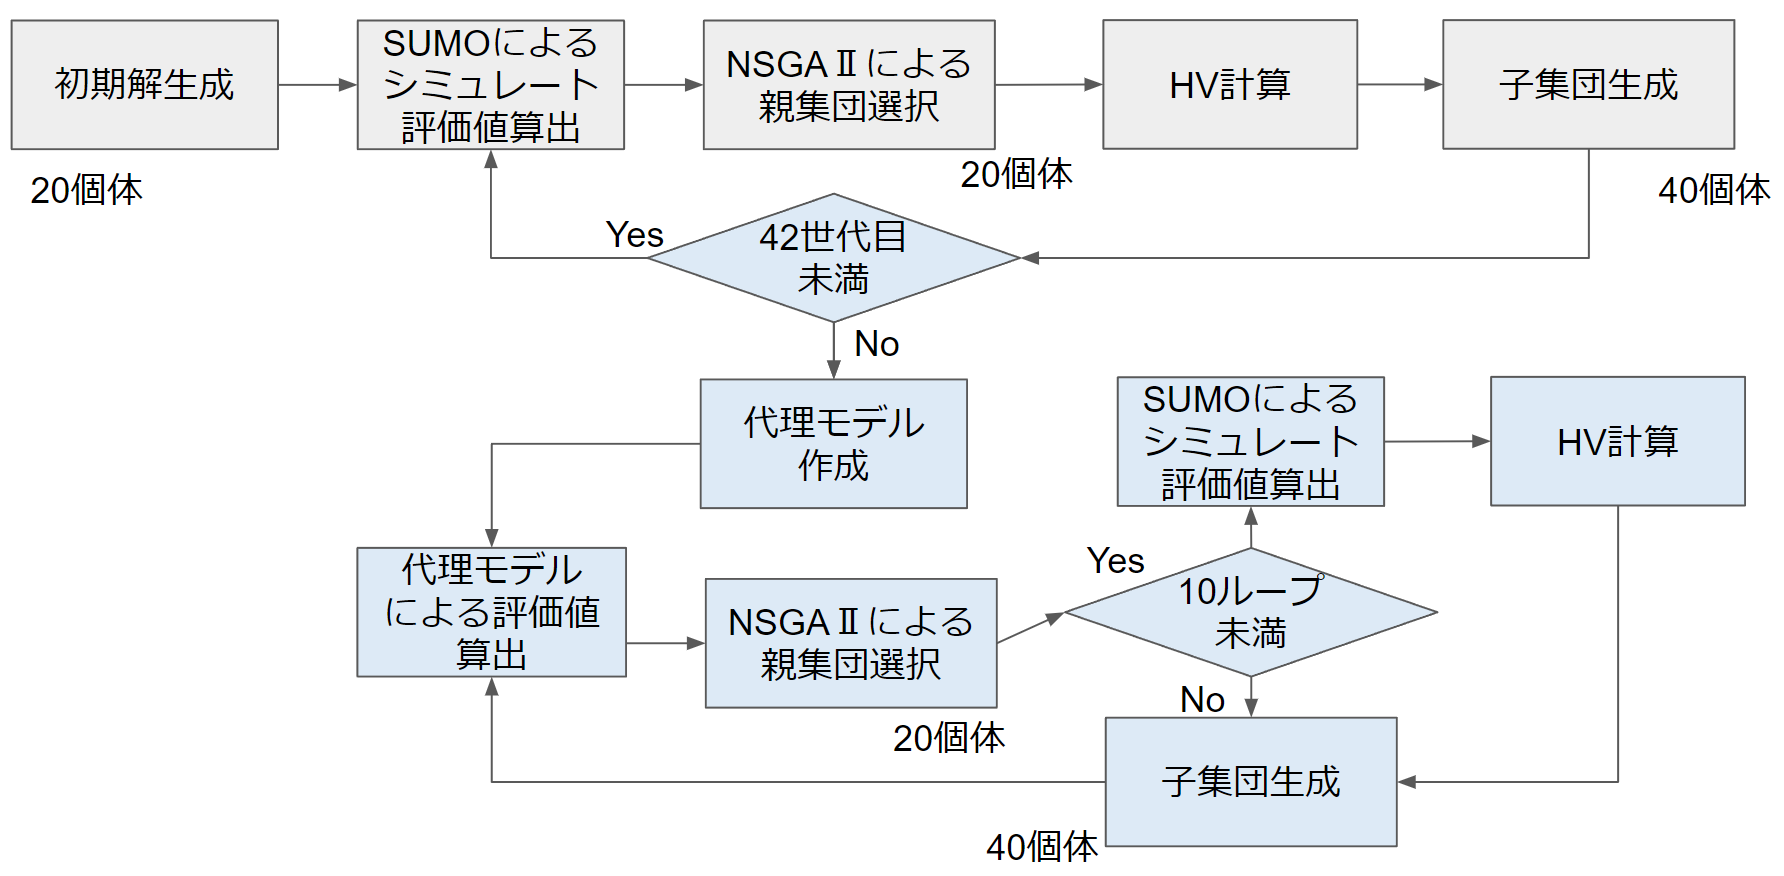
\includegraphics[width=\linewidth]{figures/d.png}
            \caption{提案手法1のフローチャート}
            \label{d}
        \end{figure}
        
        図\ref{d}で灰色の要素については図\ref{old_algo}と一致しており,青色の要素が新しく導入された要素である.
        実験3で示したように,41世代目までをWalsh関数の学習データにするため,41世代目までは先行研究と同じアルゴリズムである.
        42世代目で,Walsh関数を用いた代理モデルを作成する.
        そして,代理モデルによって評価値を算出し,親集団を選択,子集団を20個体生成,代理モデルによる評価を繰り返す.
        代理モデルを用いた親集団選択と子集団生成を10ループ行う.
        これは,代理モデルのみを用いて10世代分進化を行っていることと同値である.
        これが,この手法の特徴である.
        ただし,最終的なHVの値はSUMOによるシミュレートを用いて評価値を算出し求める.
        代理モデルを用いて10世代分進化を行い,それで得られた個体を,全体の1世代の進化とするのがこの手法である.
        ただし,この10世代という値は,なにか定量的な根拠に基づいた数字ではない点について,今後の研究課題であるといえる.
        \subsection{提案手法2}
        図\ref{k}にフローチャートを示す.
        \begin{figure}
            \centering
            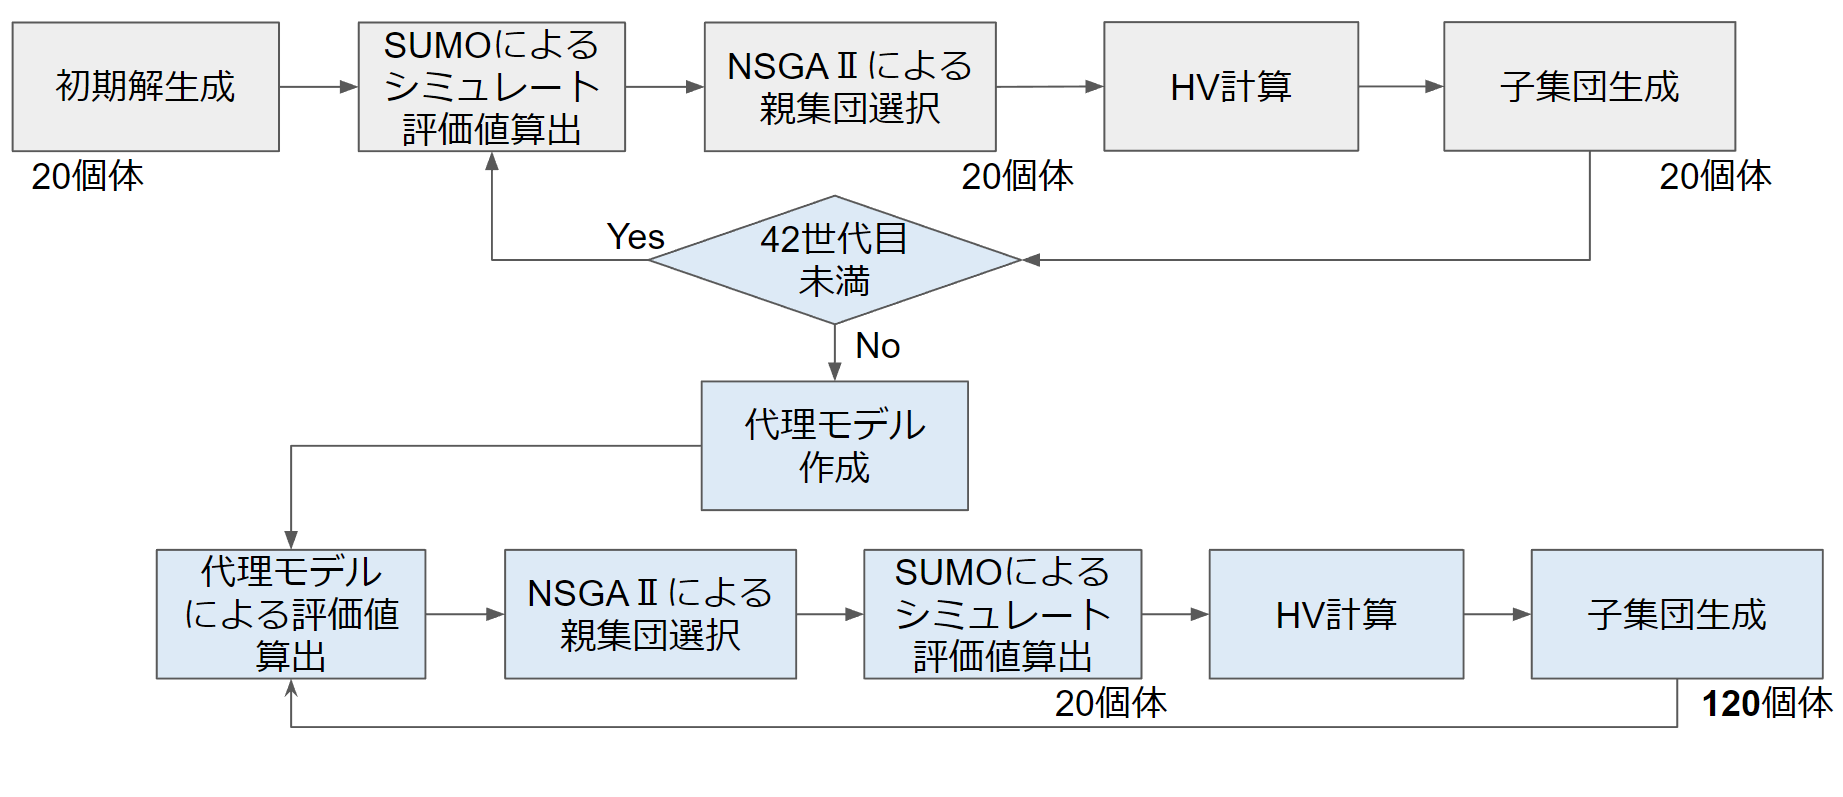
\includegraphics[width=\linewidth]{figures/k.png}
            \caption{提案手法2のフローチャート}
            \label{k}
        \end{figure}

        図\ref{k}で灰色の要素については図\ref{old_algo}と一致しており,青色の要素が新しく導入された要素である.
        青色の要素について,その要素や順番は灰色の要素とほとんど変化がない.
        変化しているところは子集団生成における,生成する子の数である.
        従来では,1世代あたり20個体子を生成していたのに対し,この手法では120個体生成している.
        120個体生成しても,代理モデルによって高速に評価できるため,問題なく親集団20個体を選択することが出来る.
        代理モデル内で進化を行うわけでなく,子集団を増やすことで多くの解を生成し,検証するのがこの手法の特徴である.
        ただし,提案手法1と同じように,120個体という値は,なにか定量的な根拠に基づいた数字ではない点について,今後の研究課題であるといえる.

        両者の手法でフローチャートには書かれていないが,1世代ごとに代理モデルは再学習され,代理モデルの精度はより上がっていく.

    \section{結果}
        \subsection{提案手法1}
        図\ref{d_result}に結果を示す.
        \begin{figure}
            \centering
            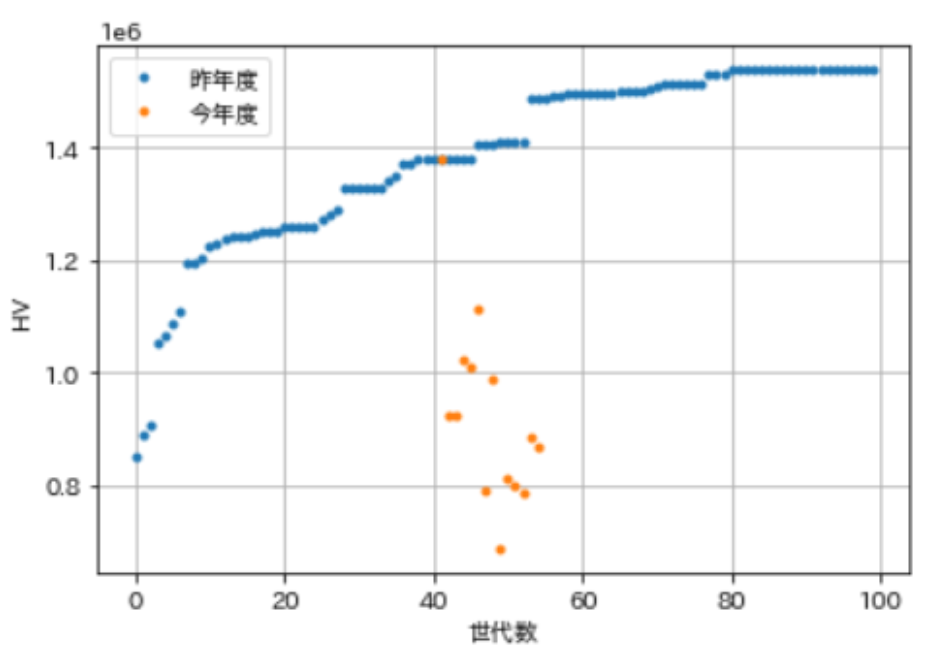
\includegraphics[width=\linewidth]{figures/d_result.png}
            \caption{提案手法1の結果}
            \label{d_result}
        \end{figure}

        43世代目以降,今年度のHVが昨年度のHVを上回ることは無かった.
        さらに,HVの値が世代ごとに大きく異なり不安定である.
        \subsection{提案手法2}
        図\ref{k_result}に結果を示す.
        \begin{figure}
            \centering
            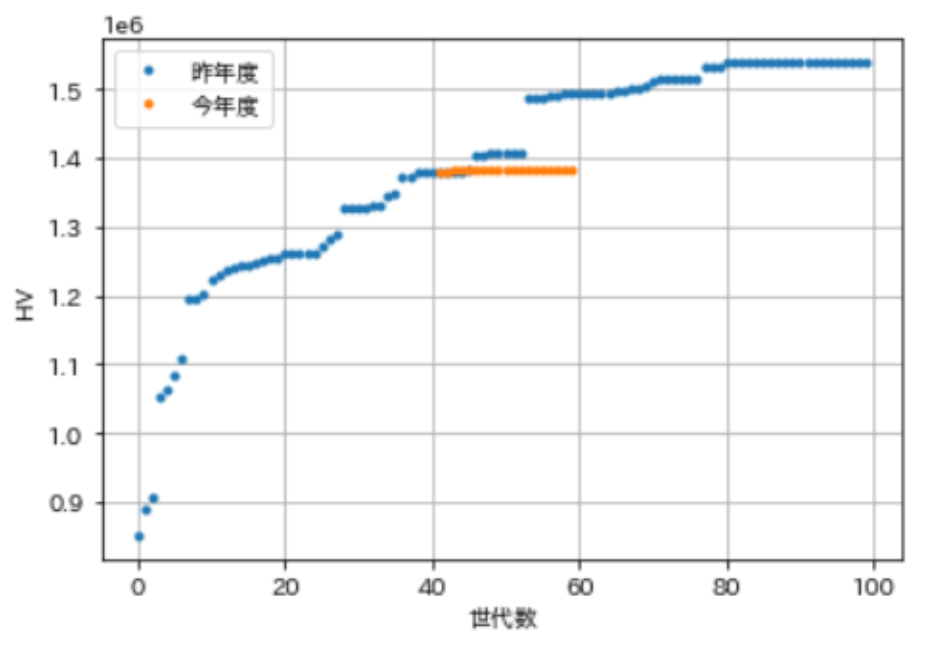
\includegraphics[width=\linewidth]{figures/k_result.png}
            \caption{提案手法2の結果}
            \label{k_result}
        \end{figure}

        提案手法1と比較して,世代ごとのHVの値が安定している.
        さらに,44\textasciitilde47世代までは今年度が昨年度のHVを上回っている.
        しかし,48世代以降は昨年度ほどの進化が進まず,HVの値は今年度が下回っている.

    \section{考察}
    代理モデルの評価値は誤差を含む.
    提案手法1では,SUMOのシミュレートによる正確な評価値を得ないまま進化を繰り返す.
    このことにより提案手法1の進化では,誤った評価値を持つ解が遺伝子として残り,
    子集団生成で誤った評価の遺伝子の特徴を受け継いだ進化を繰り返す.
    よって,HVの値が大きく下がり,かつ世代ごとにHVの値が不安定になったと考えられる.
    今回は10ループごとにHVを計算したが,このループ数を大きくすれば,よりHVは不安定になると考えられる.

    それに対し提案手法2では,誤差を含んだ代理モデルで進化を繰り返すことは無い.
    子集団を生成する過程で代理モデルを利用することは無いため,ここで誤差が生まれることは無い.
    子集団の評価は代理モデルによって行われ誤差が生まれるが,そこで親集団を選択しSUMOによる正確な評価が行われ,
    悪い特徴を持った遺伝子は悪い評価値を得るため,提案手法1に比べHVの値が安定したと考えられる.
    提案手法2では,44~47世代までは今年度が昨年度のHVを上回ることが出来た.
    昨年度アルゴリズムでは子集団を20個体しか作ることが出来ず,より優れた個体が生まれる可能性が少なかった.
    それに対し提案手法2では,子集団を120個体生成することができ,より優れた個体が生まれる可能性が昨年度より高く,
    それによりHVが昨年度を上回ったと考えられる.
    しかし,提案手法2は誤りを含む評価値を持った子集団が親集団選択されるため,本当に優れた個体が親集団に残らない可能性がある.
    これにより,48世代以降では昨年度を下回る結果になったと考えられる.



    

\end{document}